% !TeX program = xelatex
% 插入位置：2.3.2「Isaac Sim 物理模擬與場景建置」。
% 接在介紹牆面、門扇、桌面與操作物件的段落之後。
% 將 simulation_environment_map.pdf 上傳至 figsrc/ch02/。

本研究之室內模擬環境配置如\cref{fig:simulation_environment_map}所示，包含臥室、客廳與右側房間。臥室與客廳之間設置可操作門扇，客廳與右側房間則以通行開口相連；茶几與抽屜櫃分別提供物件抓取及關節式物件操作情境。各次實驗之起始條件、障礙物配置與任務設定將於第四章說明。

\begin{figure}[htbp]
    \centering
    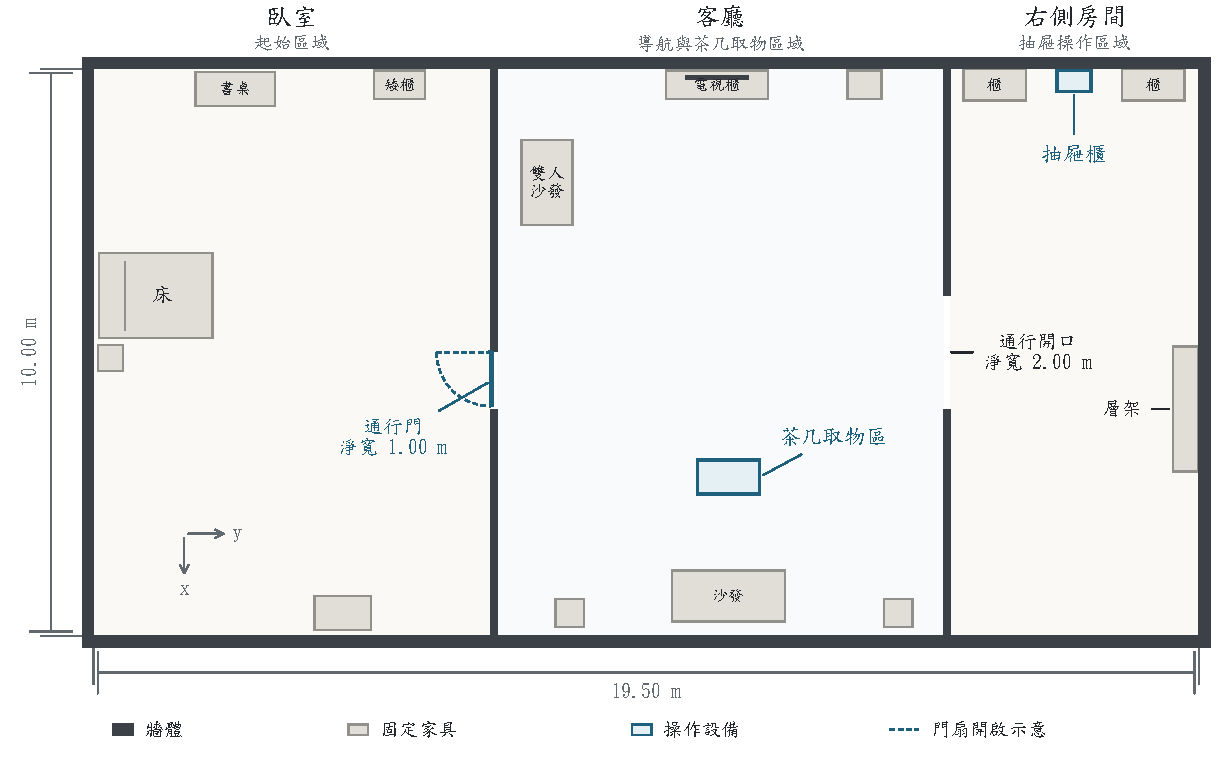
\includegraphics[width=1.0\textwidth]{figsrc/ch02/simulation_environment_map.pdf}
    \caption{室內模擬環境與任務區域配置}
    \label{fig:simulation_environment_map}
\end{figure}
